\chapter{Demonstrative Experiment}
\label{chapter:demonstrative-experiment}

This chapter presents a demonstrative simulation experiment done on the CN6880 PSE model. The goal of the experiment is to demonstrate how the queue types and priorities affect the scheduler, and hence the packet throughput and latency, and at the same time validate the scheduler functionality implemented in the model. It also demonstrates the usage of probes to detect bottlenecks in a system.

\section{Experiment Setup}
\label{sec:experiment-setup}

The experiment consists of two different simulations and measurements. We will first demonstrate a packet processing application whose throughput is limited due to the bottleneck occurring from a slow atomic processing. We will then modify the application, splitting part of the atomic processing into parallel, thus breaking the bottleneck.

Both of the simulations consist of a single packet stream, which is generated from a two level workload model. The first workload node is similar workload generator node as presented in Figure~\ref{fig:full-model}. It triggers its child node with interval $RNS\_random\_uniform(5*10^{-5}, 15*10^{-5})$ seconds, and lifetime of 0.05 seconds. The child node creates 512B packets with interval $5.1~*~10^{-8}$~$*$~$RNS\_random\_lognormal(-10, 0.9)$ seconds for $4*10^{-5}$ seconds.

Figure~\ref{fig:experiment-hardware} presents the hardware model used in the experiment. It consists of six active resources. The PKI and PKO units are consumed by the input and output phases of the packet flow, respectively. Each 32 processing cores have a L1 cache associated with it, and the L2 cache and RAM are shared between the cores. The cores are served as first come first serve basis, as the scheduling logic is taken care of in the SSO unit.

The SSO unit uses the custom scheduling functions presented in the section~\ref{sec:custom-scheduler-functions}, enabling the use of atomicity, queue priorities, and coremasks. The core release is a typical relase node referring to the SSO unit.

\begin{figure}[]
  \begin{center}
    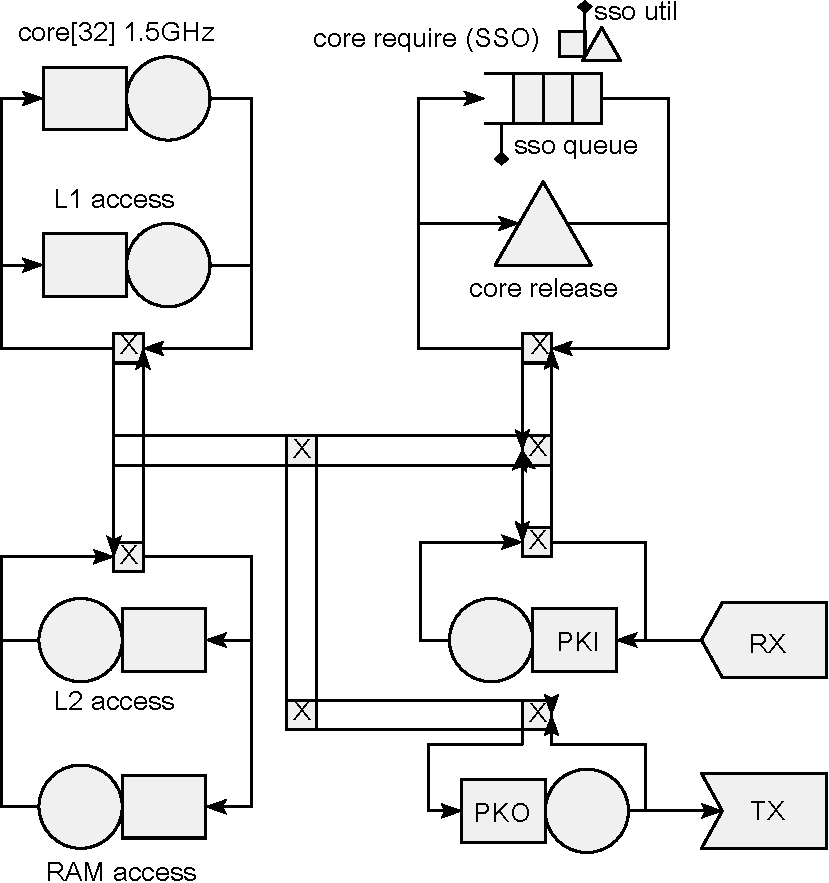
\includegraphics[width=0.6\textwidth]{images/pse-models/experiment-hardware.pdf}
    \caption{TODO}
    \label{fig:experiment-hardware}
  \end{center}
\end{figure}

The software model is presented in figure~\ref{fig:experiment-software}. The high level software model consists of the input, process, and output phases. The 'packet input' and 'packet output' nodes are modeled exactly as discussed in the section~\ref{sec:characteristic-measurements}, delaying the the packets according to the equation~\ref{eq:1}.

The two different applications used in the experiment, are shown in the software model after the 'select app' -node. The lower and upper application are referred as application 1 and application 2, respectively. The application selection is done in the workload model by the 'AppId' attribute.

The first packet processing application consists of two processing steps, both consuming CPU and memory for the range of 5000 clock cycles. The first step consists of parallel, priority 2 queue (A), and the second one is done atomically with priority 1 queue (B). The second simulation application is a modified version of the first packet processing application, where the second processing step is split into parallel and atomic steps. The release nodes are omitted from the software model for clarity.

\begin{figure}[]
  \begin{center}
    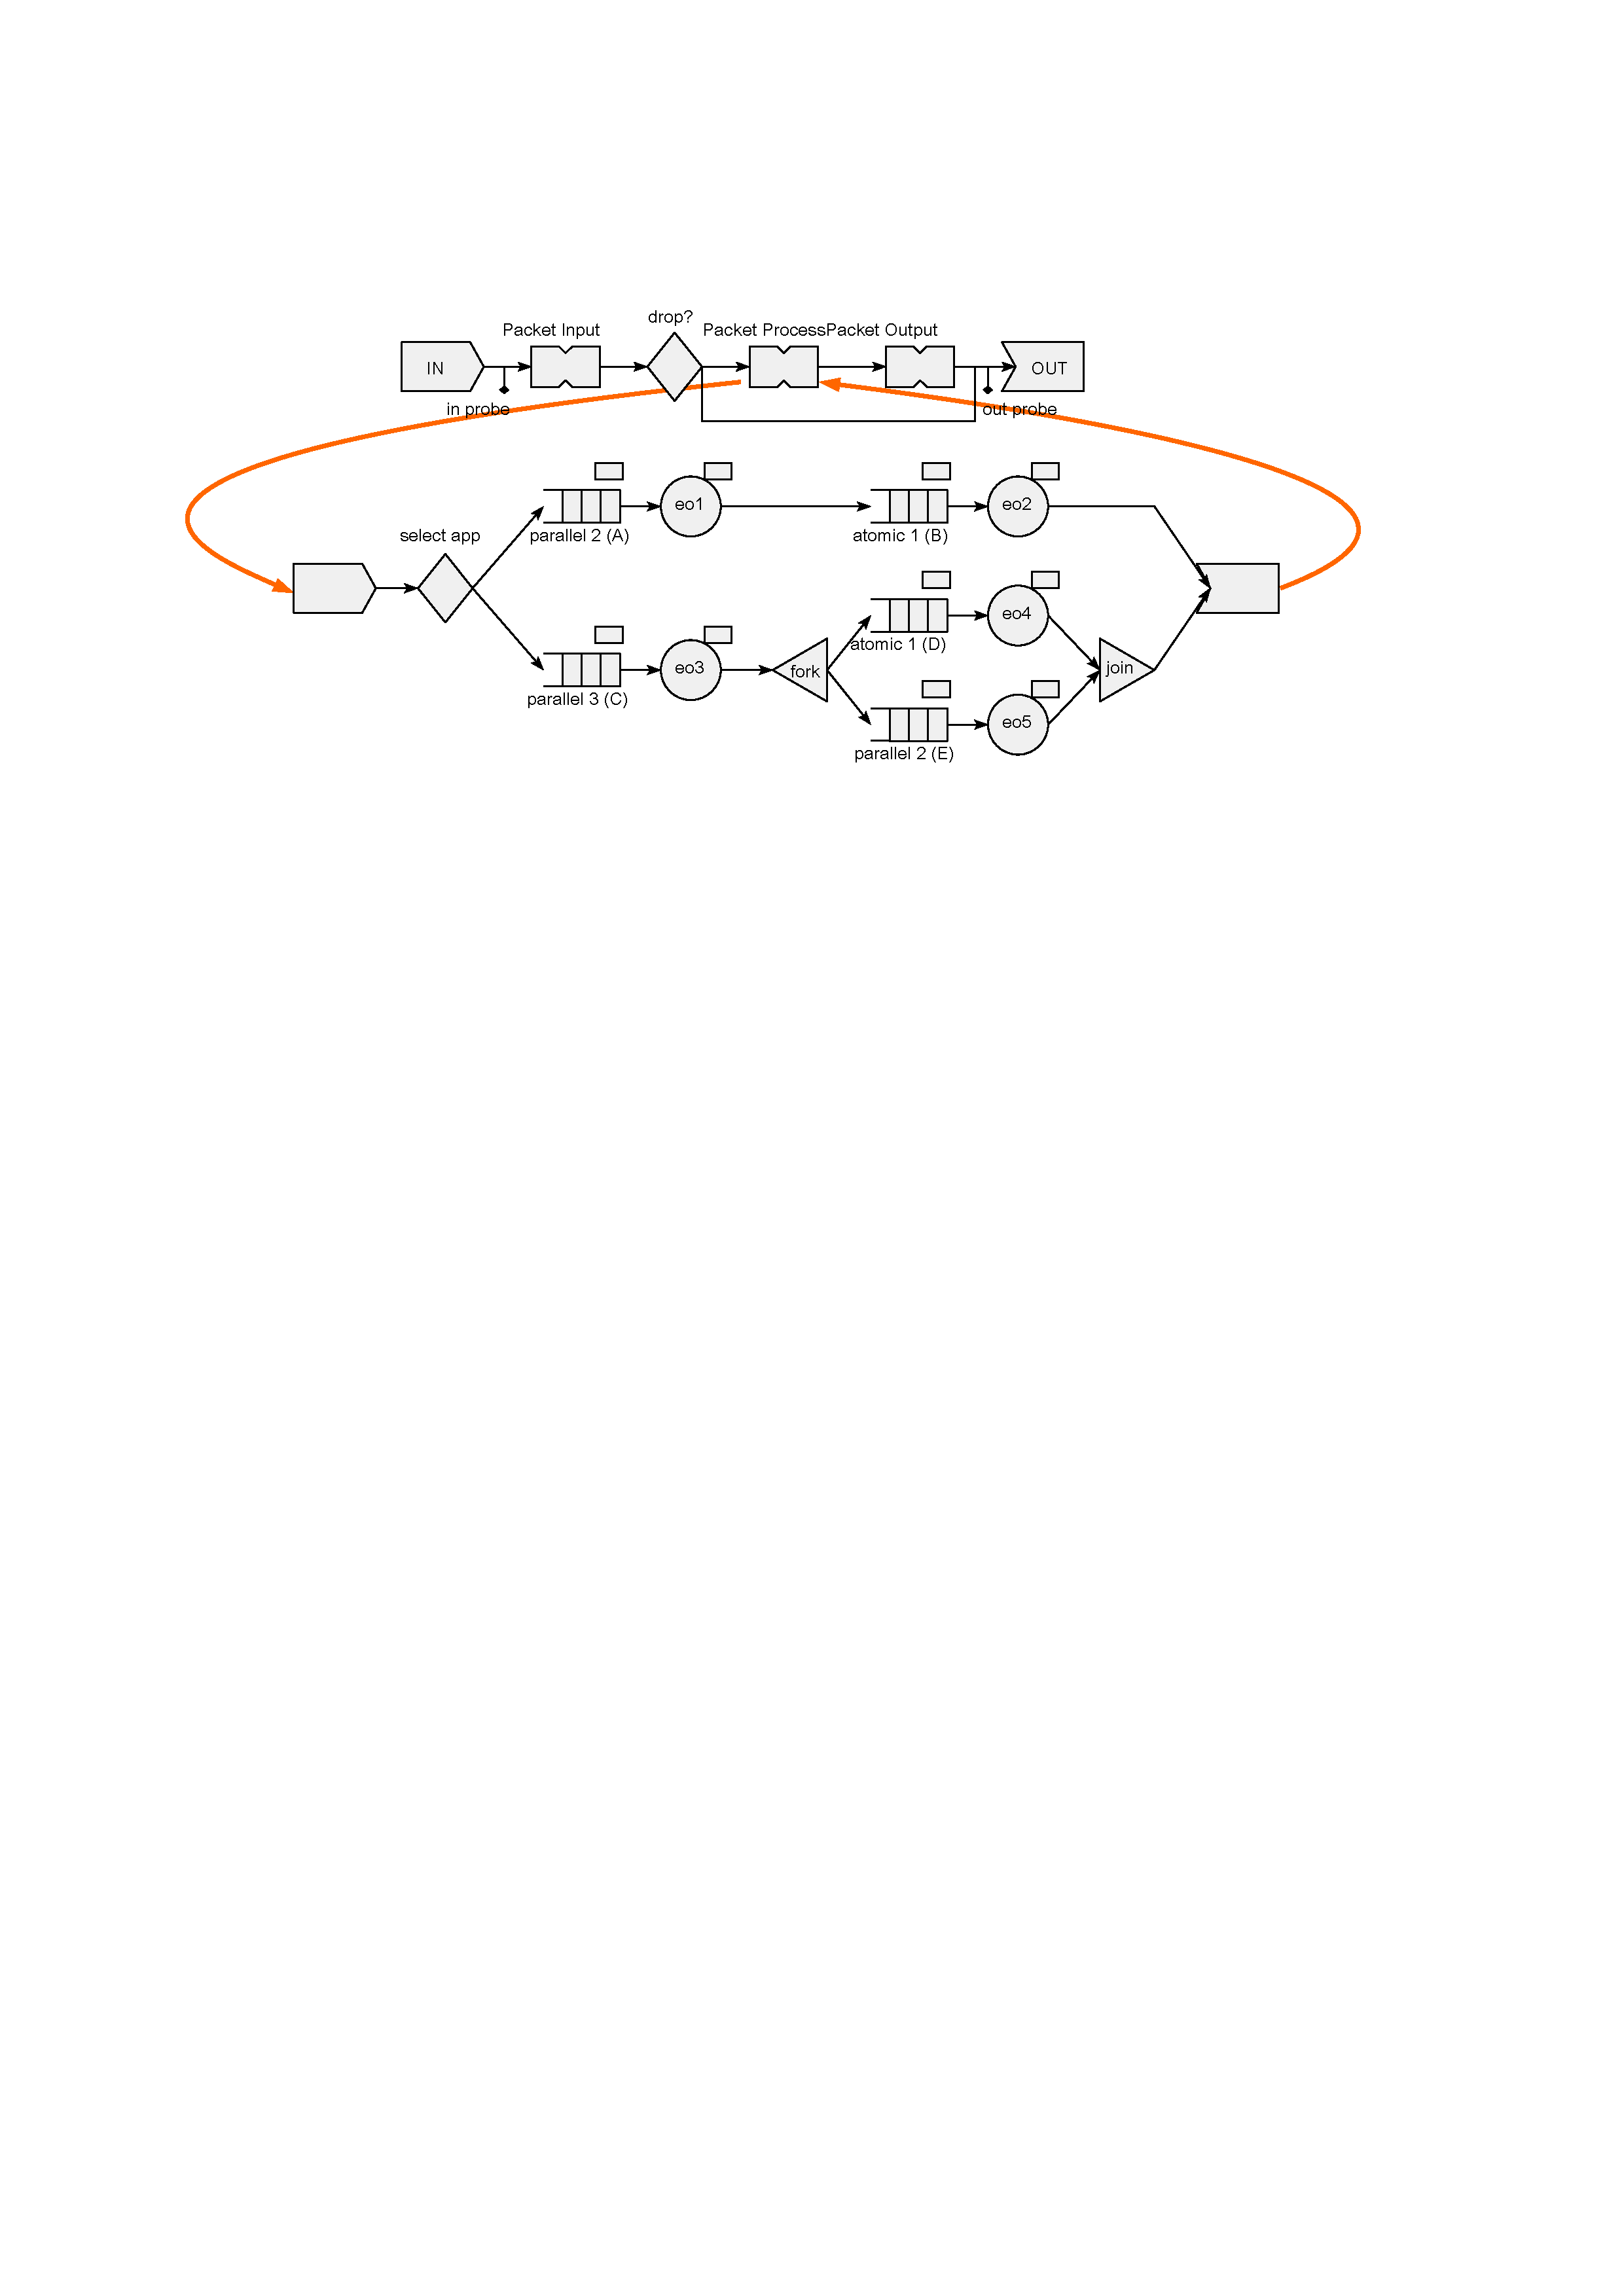
\includegraphics[width=\textwidth]{images/pse-models/experiment-software.pdf}
    \caption{TODO}
    \label{fig:experiment-software}
  \end{center}
\end{figure}

% \begin{figure}[]
%   \begin{center}
%     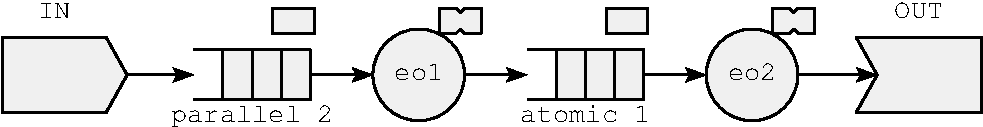
\includegraphics[width=\textwidth]{images/pse-models/application-1.pdf}
%     \caption{The example application used for the experiment. The atomic queue of eo2 produces a bottleneck to the system.}
%     \label{fig:application-1}
%   \end{center}
% \end{figure}

% \begin{figure}[]
%   \begin{center}
%     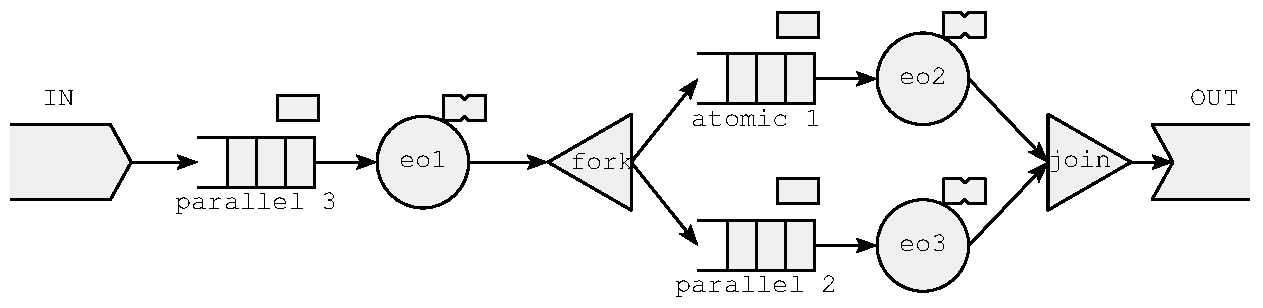
\includegraphics[width=\textwidth]{images/pse-models/application-2.pdf}
%     \caption{A modified processing application for the experiment. The bottleneck has been removed by splitting the second processing part into two.}
%     \label{fig:application-2}
%   \end{center}
% \end{figure}

We will gather two different metrics of the system. First, we are interested in the core utilization and queue lengths for each processing step. These are measured by the probes attached to the SSO unit as shown in hardware model in figure~\ref{fig:experiment-hardware}. Secondly, we are interested in the packet latencies. They are measured by calculating the time difference between the 'out probe' and the 'in probe', as shown in the software model in figure~\ref{fig:experiment-software}, for each packet.

\section{Simulation Results}
\label{sec:simulation-results}

The system was simulated twice, using both of the applications separately, and the data from the probes were post-processed. We grouped the number of tasks in the SSO/core queue, by the processing step.

Figures~\ref{fig:app1-queue2} and~\ref{fig:app1-latency} present the data from the first simulation using the packet processing application 1. Figure~\ref{fig:app1-queue2} describes the number of tasks in the SSO/core queue, that are from the atomic resource usage queue, with respect to simulation time. The corresponding graph for the first queue is omitted, as none of that tasks from it end up in the waiting queue. Figure~\ref{fig:app1-latency} presents the latency of each packet through the whole system.

\begin{figure}[]
  \begin{center}
    \includegraphics[width=\textwidth]{images/experiment/app1-queue2-crop.pdf}
    \caption{Application 1: The number of tasks in the SSO/core queue, with respect to simulation time, from the second resource usage queue.}
    \label{fig:app1-queue2}
  \end{center}
\end{figure}

\begin{figure}[]
  \begin{center}
    \includegraphics[width=\textwidth]{images/experiment/app1-latency-crop.pdf}
    \caption{Application 1: Latency of the packets through the system.}
    \label{fig:app1-latency}
  \end{center}
\end{figure}

As shown in the figures, the second processing step produces a bottleneck to the system. The processing in the second execution object is so heavy that the tasks accumulate into the waiting queue, and thus the packet latency keeps growing until the workload ceases.

The second application removes this problem by parallelizing part of the atomic processing. Figures~\ref{fig:app2-queue2} and~\ref{fig:app2-latency} present the data from the second application simulation. Figure~\ref{fig:app2-queue2} shows the number of tasks in the SSO/core queue, that are from the atomic resource usage queue, with respect to simulation time. Figure~\ref{fig:app2-latency} presents the latency of the packets through the whole system. Neither of the parallel queues have tasks in the waiting queue of the SSO/core during the simulation.

\begin{figure}[]
  \begin{center}
    \includegraphics[width=\textwidth]{images/experiment/app2-queue2-crop.pdf}
    \caption{Application 2: The number of tasks in the SSO/core queue, from the second resource usage queue.}
    \label{fig:app2-queue2}
  \end{center}
\end{figure}

\begin{figure}[]
  \begin{center}
    \includegraphics[width=\textwidth]{images/experiment/app2-latency-crop.pdf}
    \caption{Application 2: Latency of the packets through the system.}
    \label{fig:app2-latency}
  \end{center}
\end{figure}

As the figures show, the second application removes the bottleneck from the system. The latencies stay within 22$\mu$s, and the limiting queue length is always below 40, over the simulation period.

\section{Discoveries}

The experiment presents an example usage of the PSE's plugin code mechanism and simulation of network processing unit. The simulation results are encouraging. First, they show that PSE can be used for performance analysis of more complex hardware accelerated systems. This brings advantages especially in the early design space exploration, when there are no real life system available, or when individual system parameters are explored.

The plugin code mechanism extends to any resource network based simulation task, providing flexibility, and allowing even more complex systems to be modeled.

%%% Local Variables:
%%% mode: latex
%%% TeX-master: "thesis-hartikainen"
%%% End:
